\FloatBarrier\section{Dataset, categorías y análisis descriptivo}

\subsection{Origen y naturaleza de HAM10000}
HAM10000 significa \textit{Human Against Machine with 10000 training images}. Su publicación describe 10\,015 imágenes dermatoscópicas procedentes de series austríacas y australianas, obtenidas bajo condiciones de adquisición distintas \cite{tschandl2018,codella2019}. Los diagnósticos se agrupan en siete categorías y su verificación no utiliza una única vía para todas las muestras: incluye histopatología (\texttt{histo}: 5\,340 registros, 53.32\%), seguimiento digital (\texttt{follow\_up}: 3\,704, 36.98\%), consenso experto (\texttt{consensus}: 902, 9.01\%) y microscopía confocal (\texttt{confocal}: 69, 0.69\%).

Esta heterogeneidad exige dos cuidados. Primero, no debe afirmarse que todas las etiquetas proceden de biopsia. Segundo, una red podría aprender correlaciones con dispositivo, iluminación o localización además de características de la lesión. Un resultado interno favorable no demuestra que el comportamiento se mantenga en otras poblaciones, hospitales o cámaras.

\subsection{Taxonomía utilizada}
\begin{table}[htbp]\centering\small
\caption{Categorías diagnósticas del experimento y perfil clínico resumido en HAM10000.}
\begin{tabularx}{\textwidth}{@{}ll>{\raggedright\arraybackslash}Xrr@{}}
\toprule
\textbf{Código} & \textbf{Naturaleza} & \textbf{Interpretación clínica resumida} & \textbf{Imágenes} & \textbf{\% Total} \\ \midrule
\texttt{akiec} & Premaligna / in situ & Queratosis actínicas y carcinoma intraepitelial / enfermedad de Bowen. & 327 & 3.27\% \\
\texttt{bcc} & Maligna & Carcinoma basocelular. & 514 & 5.13\% \\
\texttt{bkl} & Benigna & Lesiones de tipo queratosis benigna; agrupación clínica heterogénea. & 1\,099 & 10.97\% \\
\texttt{df} & Benigna & Dermatofibroma benigno. & 115 & 1.15\% \\
\texttt{mel} & Maligna & Melanoma; incluye variantes presentes en la colección. & 1\,113 & 11.11\% \\
\texttt{nv} & Benigna & Nevus melanocítico benigno. & 6\,705 & 66.95\% \\
\texttt{vasc} & Benigna / vascular & Lesiones vasculares incluidas en el conjunto. & 142 & 1.42\% \\
\bottomrule
\end{tabularx}
\end{table}

Aunque la distribución de Kaggle se denomina \textit{Skin Cancer MNIST}, no contiene únicamente lesiones malignas y no es el MNIST de dígitos. Los CSV de $8\times 8$ y $28\times 28$ píxeles son derivados de baja resolución. El proyecto utiliza los JPEG originales ($600\times 450$ píxeles) y sus etiquetas oficiales, no esas matrices reducidas, porque las estructuras dermatoscópicas finas se pierden al reducir drásticamente la resolución.

\subsection{Archivos y relación con las etiquetas}
Las carpetas \texttt{HAM10000\_images\_part\_1} y \texttt{HAM10000\_images\_part\_2} contienen 5\,000 y 5\,015 imágenes, respectivamente. Son lotes de distribución de un único dataset, no dos clases ni una separación \texttt{train/test}. Las etiquetas se obtienen uniendo el nombre del archivo con la columna \texttt{image\_id} de \texttt{HAM10000\_metadata.csv}. La columna objetivo es \texttt{dx}, mientras que \texttt{lesion\_id} identifica una lesión física y permite agrupar sus distintas tomas.

La versión del ZIP inicialmente descargada repetía ambos lotes con diferencias de mayúsculas en el nombre de las carpetas. Esa duplicación de empaquetado se eliminó al generar el archivo limpio (\texttt{2770.8~MiB}). Es un problema distinto de los registros binarios duplicados encontrados dentro de las 10\,015 muestras legítimamente indexadas por el metadata. No deben confundirse ambos fenómenos.

\subsection{Distribución, desbalance e inspección visual}
\begin{table}[htbp]\centering\normalsize
\setlength{\tabcolsep}{8pt}
\caption{Distribución verificada del conjunto HAM10000 por clase y lesión única.}
\begin{tabularx}{0.92\textwidth}{>{\raggedright\arraybackslash}Xrrr}\toprule
\textbf{Clase} & \textbf{Imágenes} & \textbf{Lesiones únicas} & \textbf{Porcentaje} \\ \midrule
\texttt{akiec} & 327 & 228 & 3.27\% \\
\texttt{bcc} & 514 & 327 & 5.13\% \\
\texttt{bkl} & 1\,099 & 727 & 10.97\% \\
\texttt{df} & 115 & 73 & 1.15\% \\
\texttt{mel} & 1\,113 & 614 & 11.11\% \\
\texttt{nv} & 6\,705 & 5\,403 & 66.95\% \\
\texttt{vasc} & 142 & 98 & 1.42\% \\
\midrule
\textbf{Total} & \textbf{10\,015} & \textbf{7\,470} & \textbf{100.00\%} \\
\bottomrule\end{tabularx}\end{table}


La categoría \texttt{nv} representa aproximadamente dos tercios del conjunto (66.95\%), mientras que \texttt{df} contiene apenas 115 imágenes (razón $58.3:1$). Un predictor trivial que siempre entregue \texttt{nv} alcanzaría una exactitud cercana al 67\% sin resolver ninguna de las demás categorías. Esta referencia explica por qué se elige Macro F1 como métrica principal y se exige analizar \textit{recall} y errores por clase. Las Figuras~\ref{fig:clases} y~\ref{fig:lesiones} muestran la distribución absoluta por imagen y su comparación frente a los conteos por lesión única.

\begin{figure}[htbp]
\centering
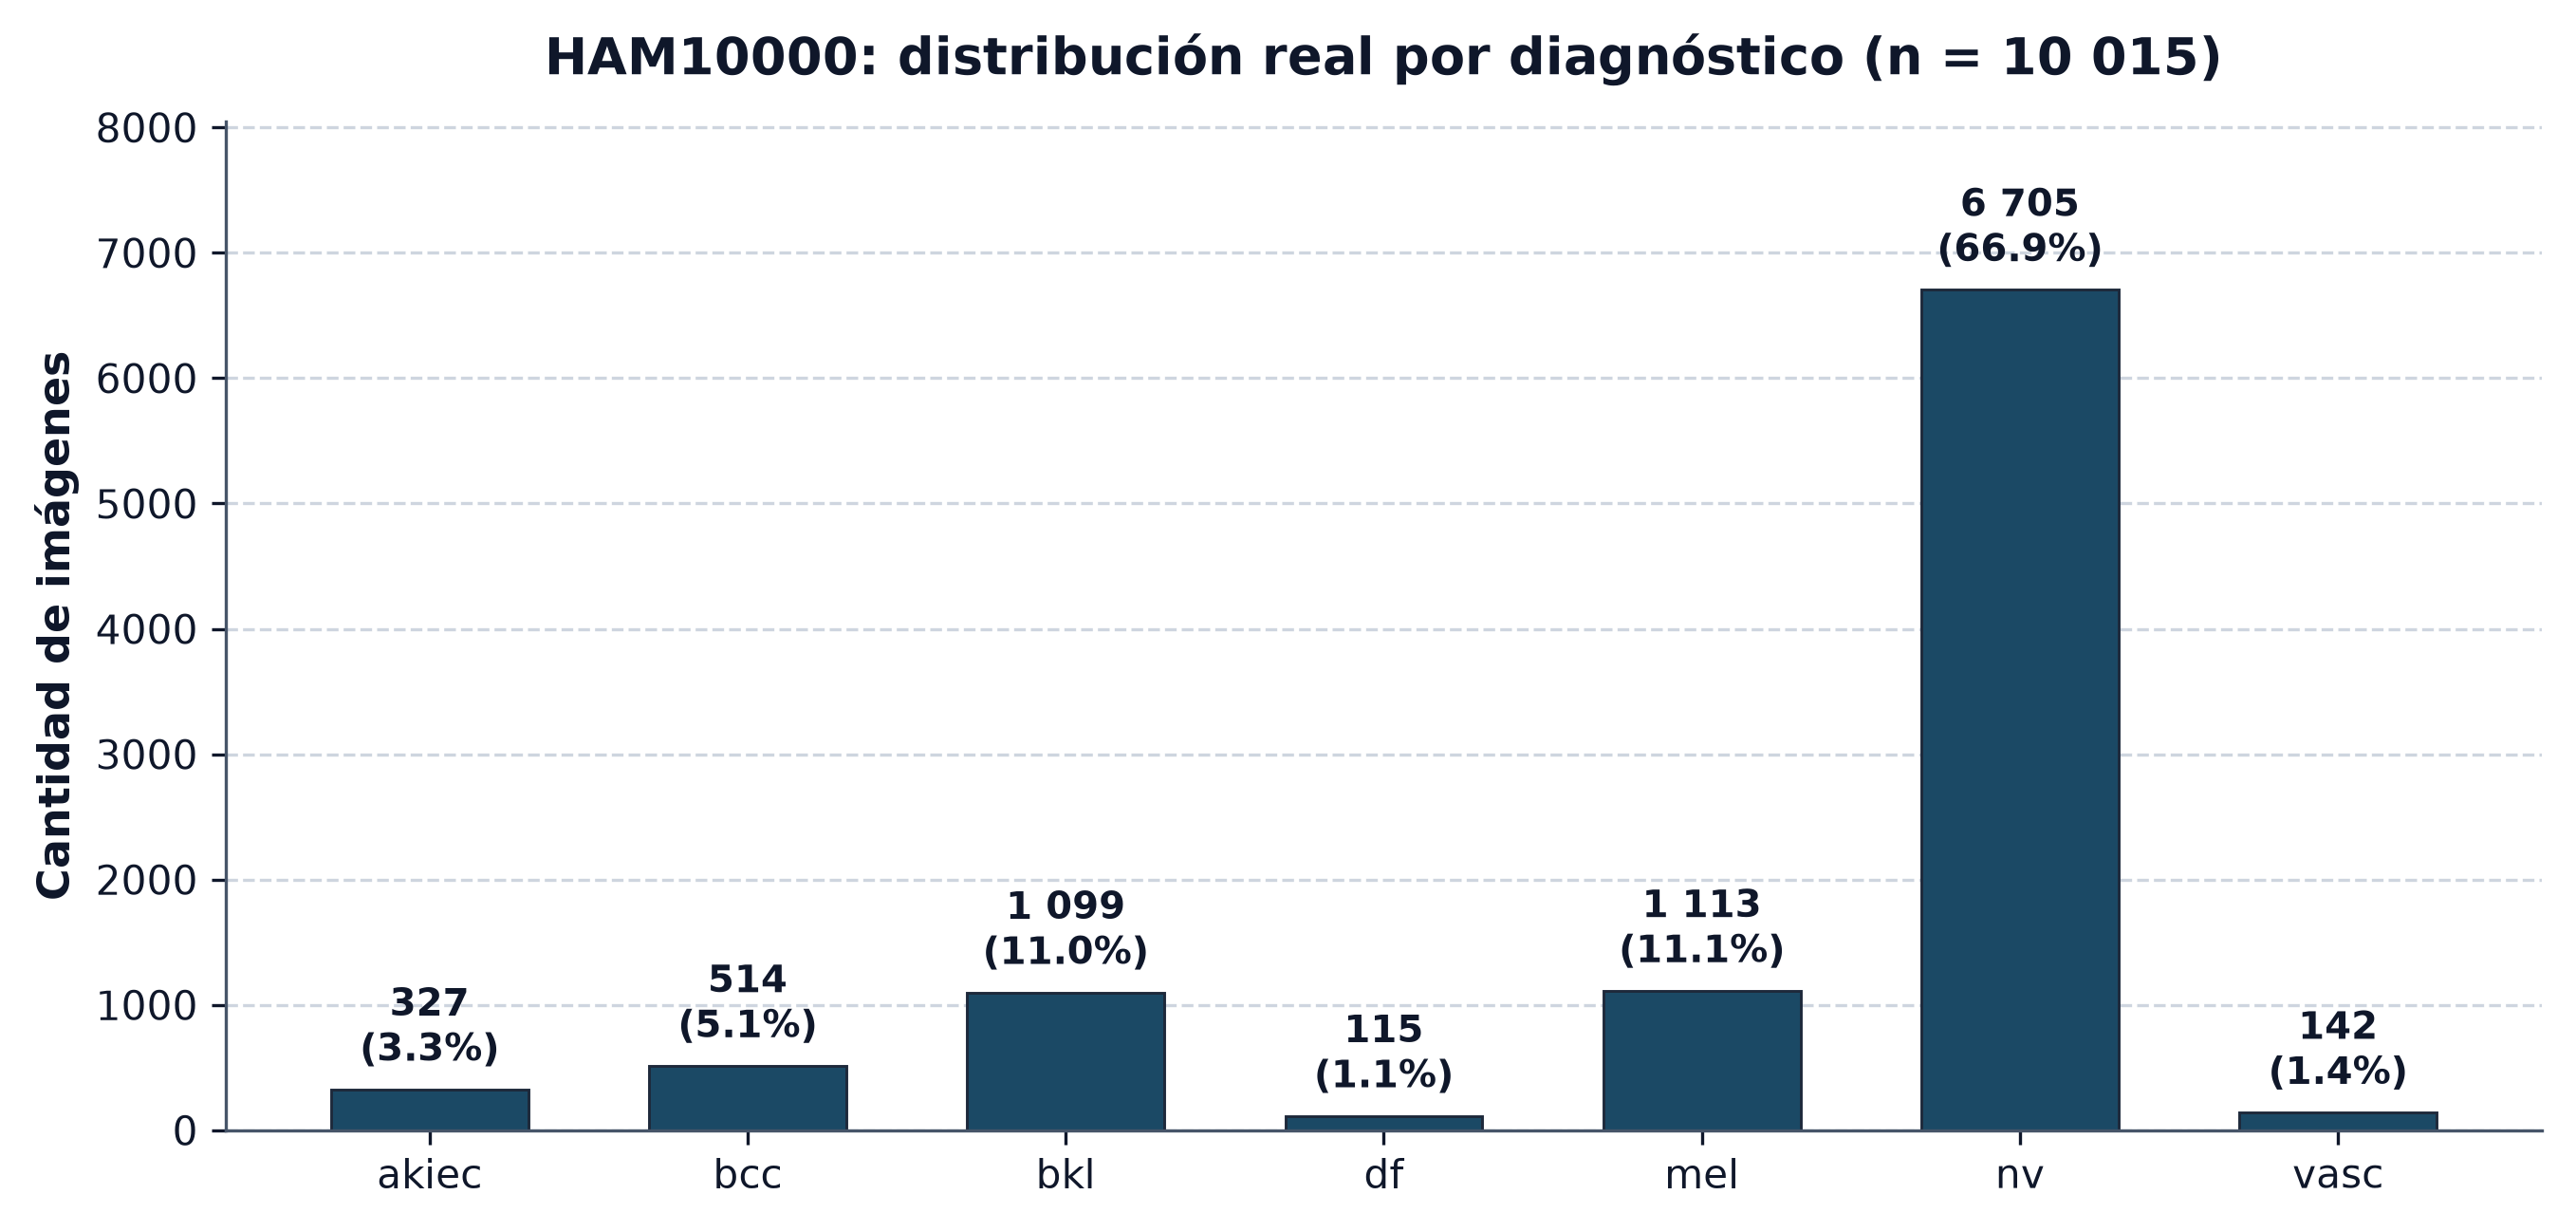
\includegraphics[width=0.92\textwidth]{01_clases.png}
\caption{Conteos y porcentajes reales por clase sobre el metadata local de HAM10000 ($n=10\,015$ imágenes). No representan métricas de desempeño de una CNN.}
\label{fig:clases}
\end{figure}

\begin{figure}[htbp]
\centering
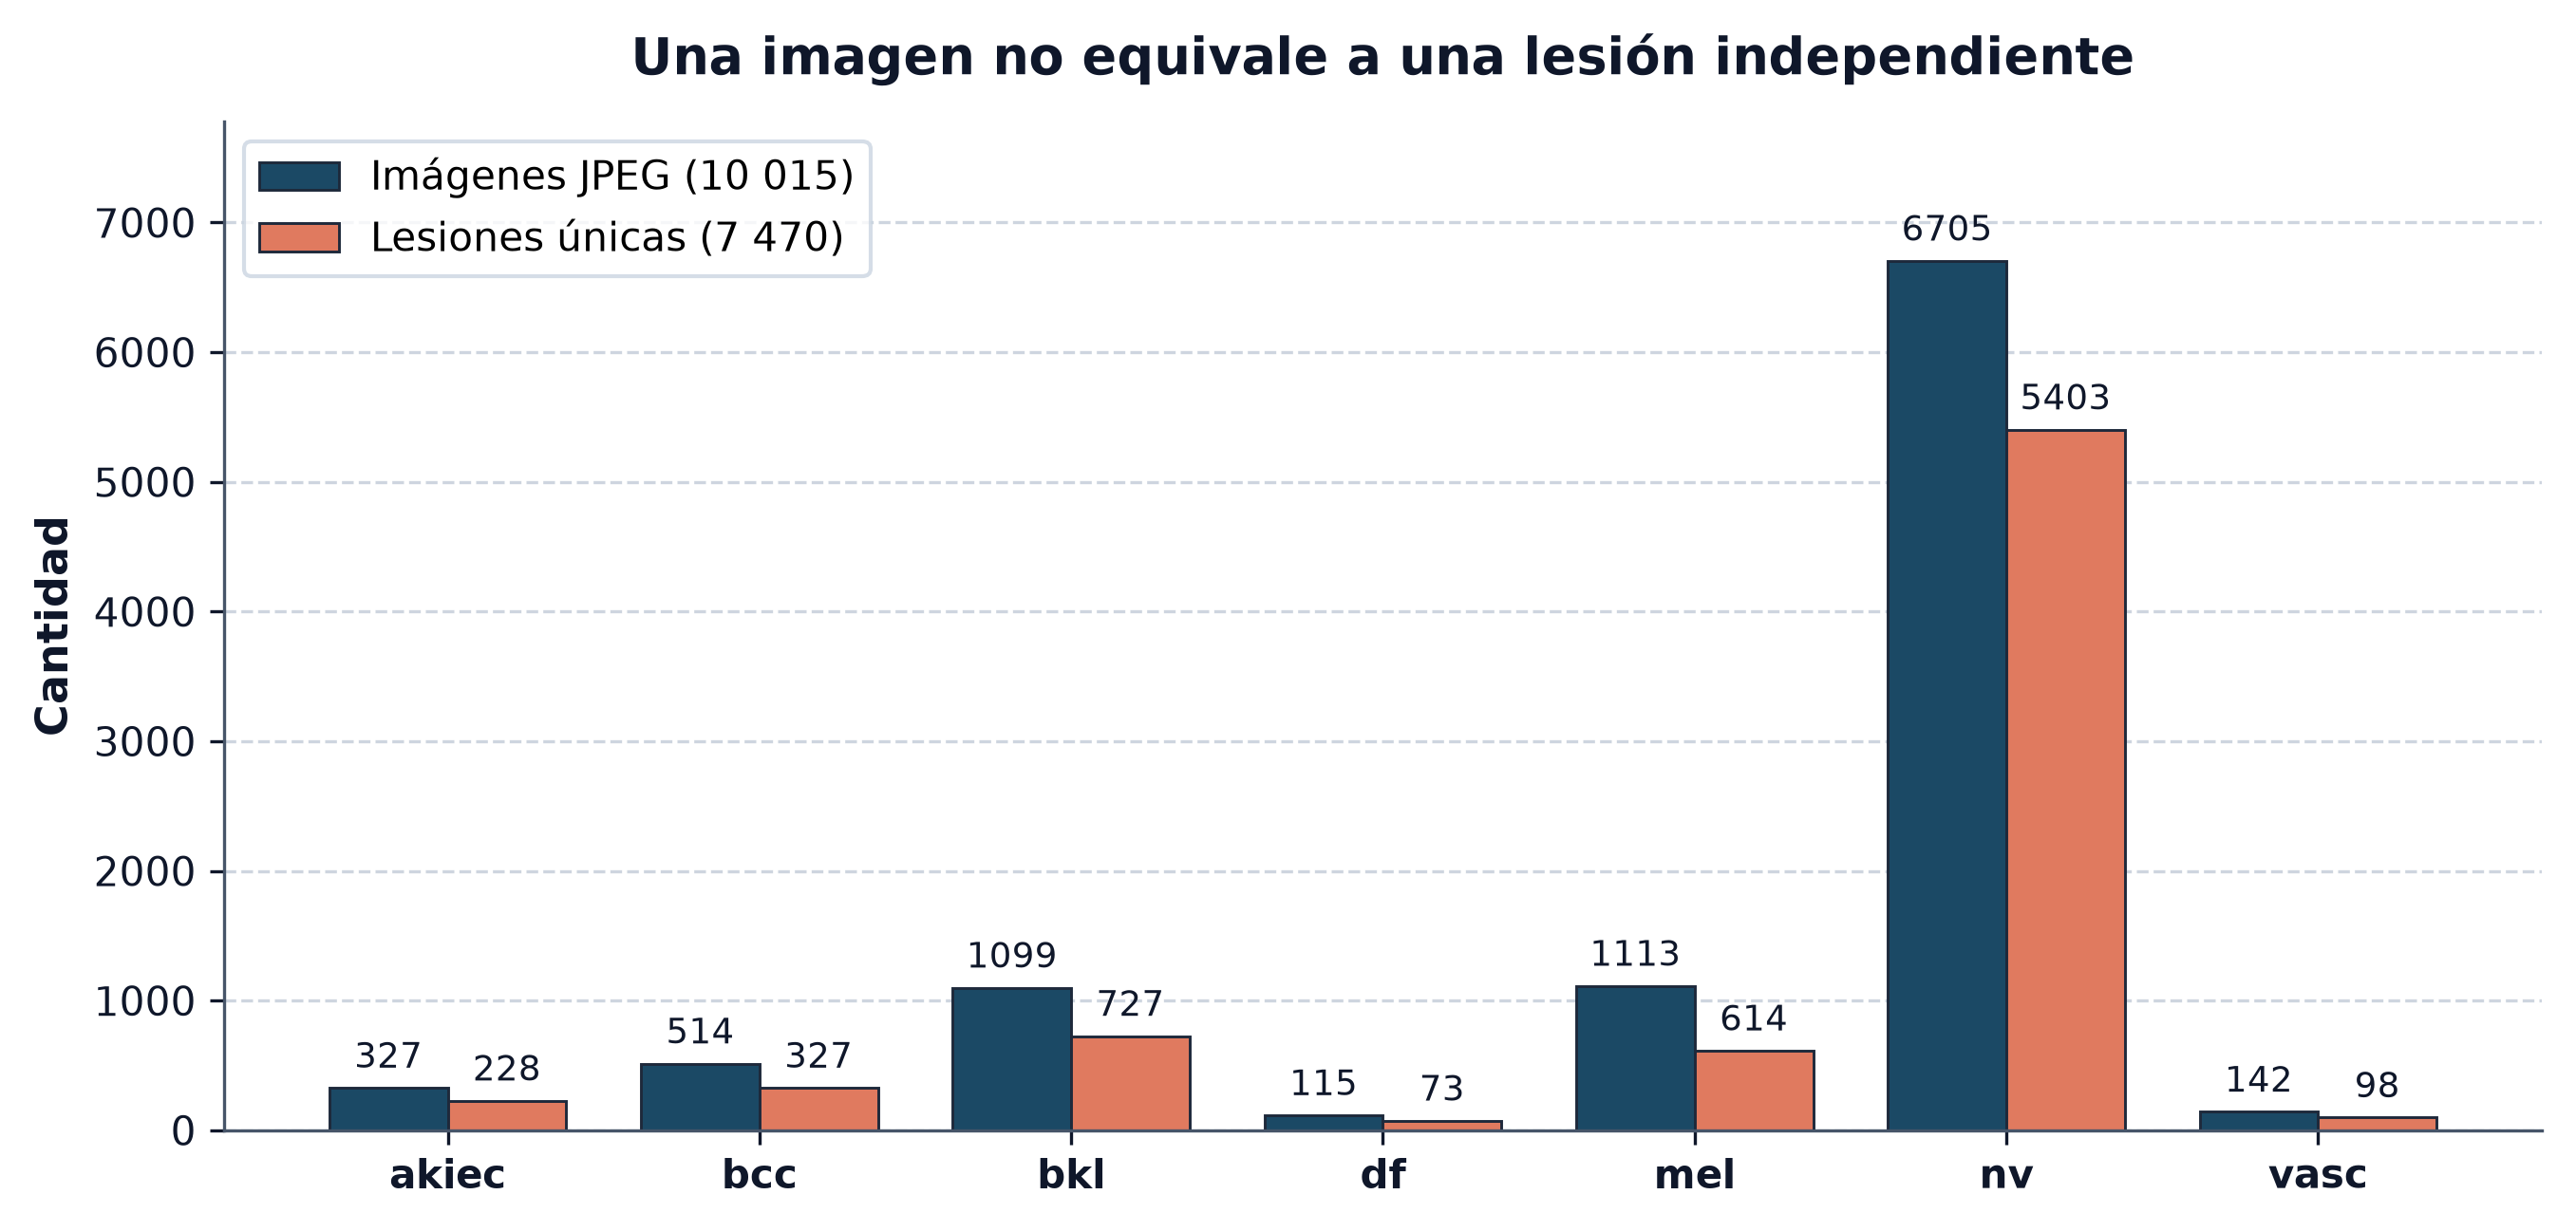
\includegraphics[width=0.92\textwidth]{02_lesiones.png}
\caption{Comparación entre número de imágenes y número de lesiones únicas (\texttt{lesion\_id}, $7\,470$ en total) por categoría diagnóstica en HAM10000.}
\label{fig:lesiones}
\end{figure}

Para ilustrar la variabilidad morfológica de entrada sin exponer muestras de validación ni prueba, la Figura~\ref{fig:muestras} presenta dos ejemplos por categoría pertenecientes exclusivamente al subconjunto de entrenamiento. Se observan diferencias en coloración, bordes, vello y marcas ópticas que justifican un preprocesamiento conservador y evaluación robusta.

\begin{figure}[p]
\centering
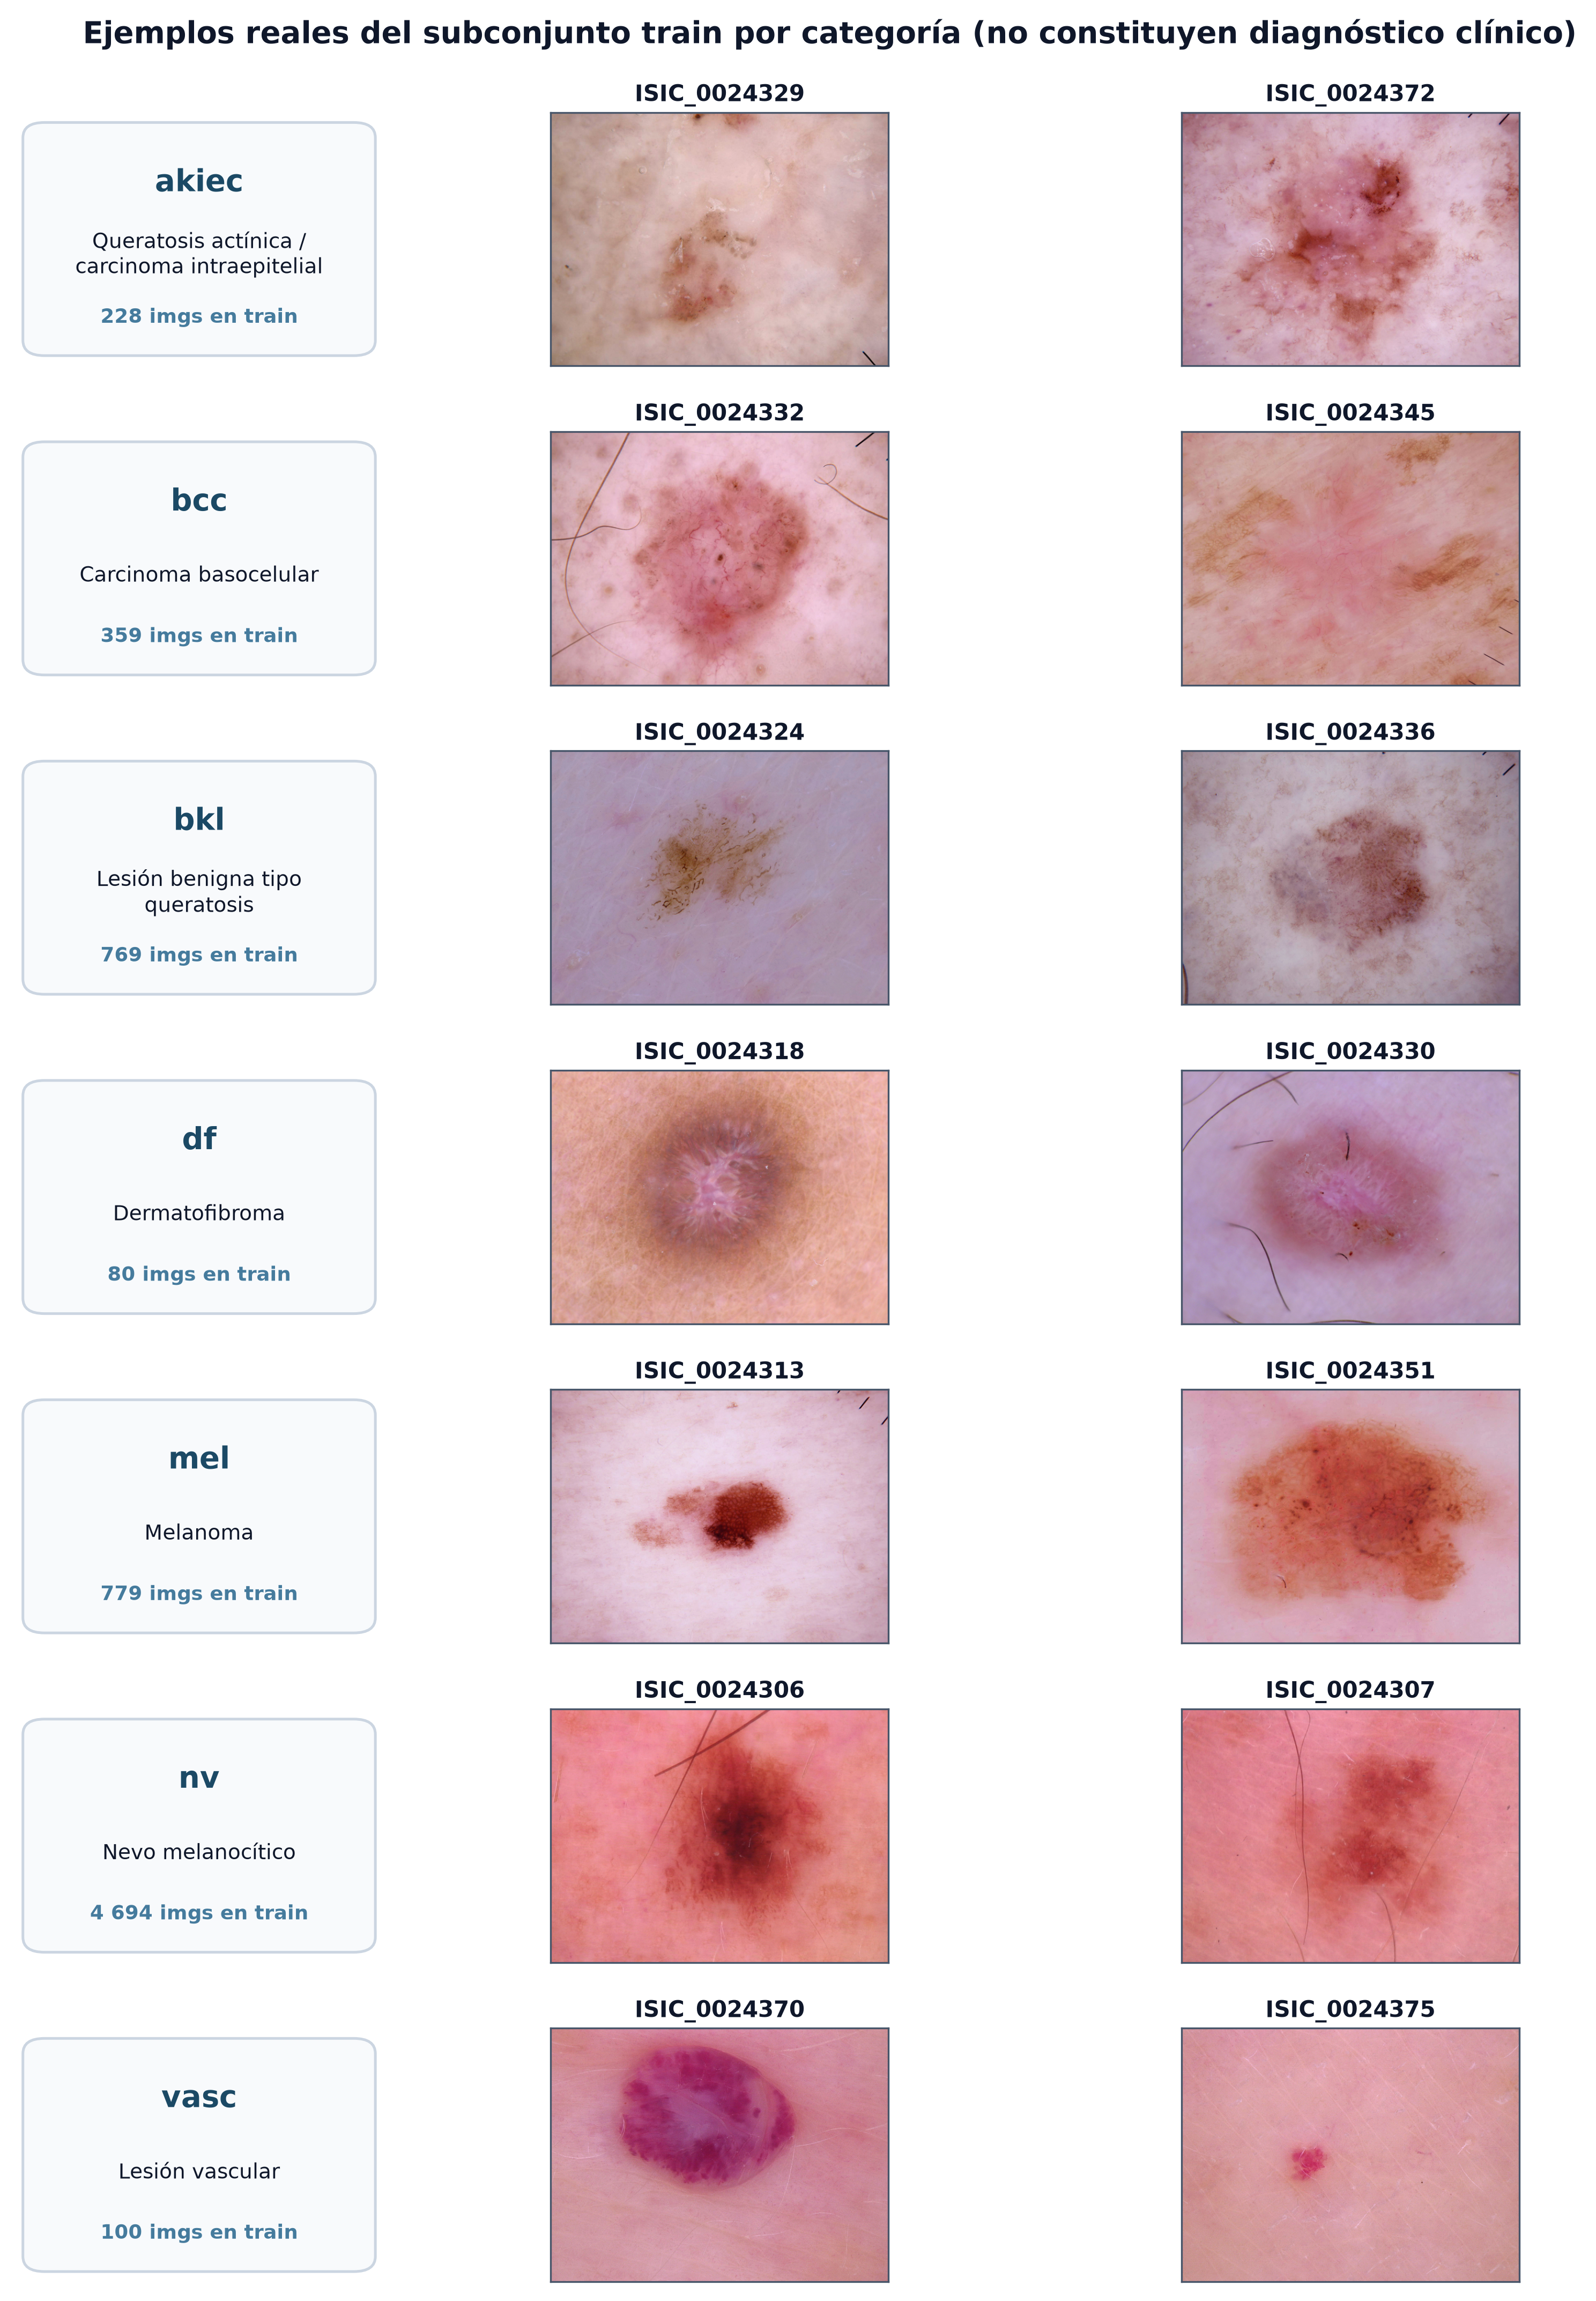
\includegraphics[width=0.94\textwidth,height=0.82\textheight,keepaspectratio]{03_muestras.png}
\caption{Dos ejemplos reales por categoría tomados únicamente de \texttt{train}. La apariencia de una imagen aislada no autoriza un diagnóstico clínico.}
\label{fig:muestras}
\end{figure}

\FloatBarrier
\subsection{Metadatos clínicos y sesgos observables}
Edad, sexo registrado y localización anatómica permiten describir la colección, pero no se utilizan como entradas en la comparación principal. Así se evita introducir una variante multimodal adicional que dificultaría atribuir diferencias de desempeño a la arquitectura visual. Los valores desconocidos o ausentes no se convierten en valores clínicos inventados.

\begin{table}[htbp]\centering\small
\caption{Resumen descriptivo de los metadatos observados en los 10\,015 registros.}
\begin{tabularx}{\textwidth}{@{}>{\bfseries\raggedright\arraybackslash}p{4.0cm}>{\raggedright\arraybackslash}p{5.0cm}>{\raggedright\arraybackslash}X@{}}
\toprule
\textbf{Atributo de metadata} & \textbf{Valores observados} & \textbf{Implicación metodológica} \\ \midrule
Edad (\texttt{age}) & Rango $[0, 85]$ años; media 51.9; 57 ausentes & Contabilizada por imagen; excluye valores faltantes sin imputación clínica. \\
Sexo (\texttt{sex}) & 5\,406 \texttt{male}, 4\,552 \texttt{female}, 57 \texttt{unknown} & Desequilibrio moderado; refleja imágenes registradas, no pacientes únicos. \\
Localización & 15 zonas (\texttt{back}: 2\,192, \texttt{lower ext.}: 2\,077, \texttt{trunk}: 1\,404) & Posible correlación de contexto visual; no se usa como variable auxiliar. \\
Verificación (\texttt{dx\_type}) & \texttt{histo} (5\,340), \texttt{follow\_up} (3\,704), \texttt{consensus} (902), \texttt{confocal} (69) & Las etiquetas no proceden únicamente de biopsia histopatológica. \\
\bottomrule
\end{tabularx}
\end{table}

Los histogramas de las Figuras~\ref{fig:metadata} y~\ref{fig:localizacion} contabilizan imágenes, no sujetos independientes. Una lesión puede contribuir varias veces y el archivo no proporciona un identificador de paciente ni una etiqueta explícita de fototipo cutáneo. La procedencia de la colección y su selección clínica limitan la generalización externa; esa limitación se debe declarar incluso si las métricas internas resultaran altas.

\begin{figure}[htbp]
\centering
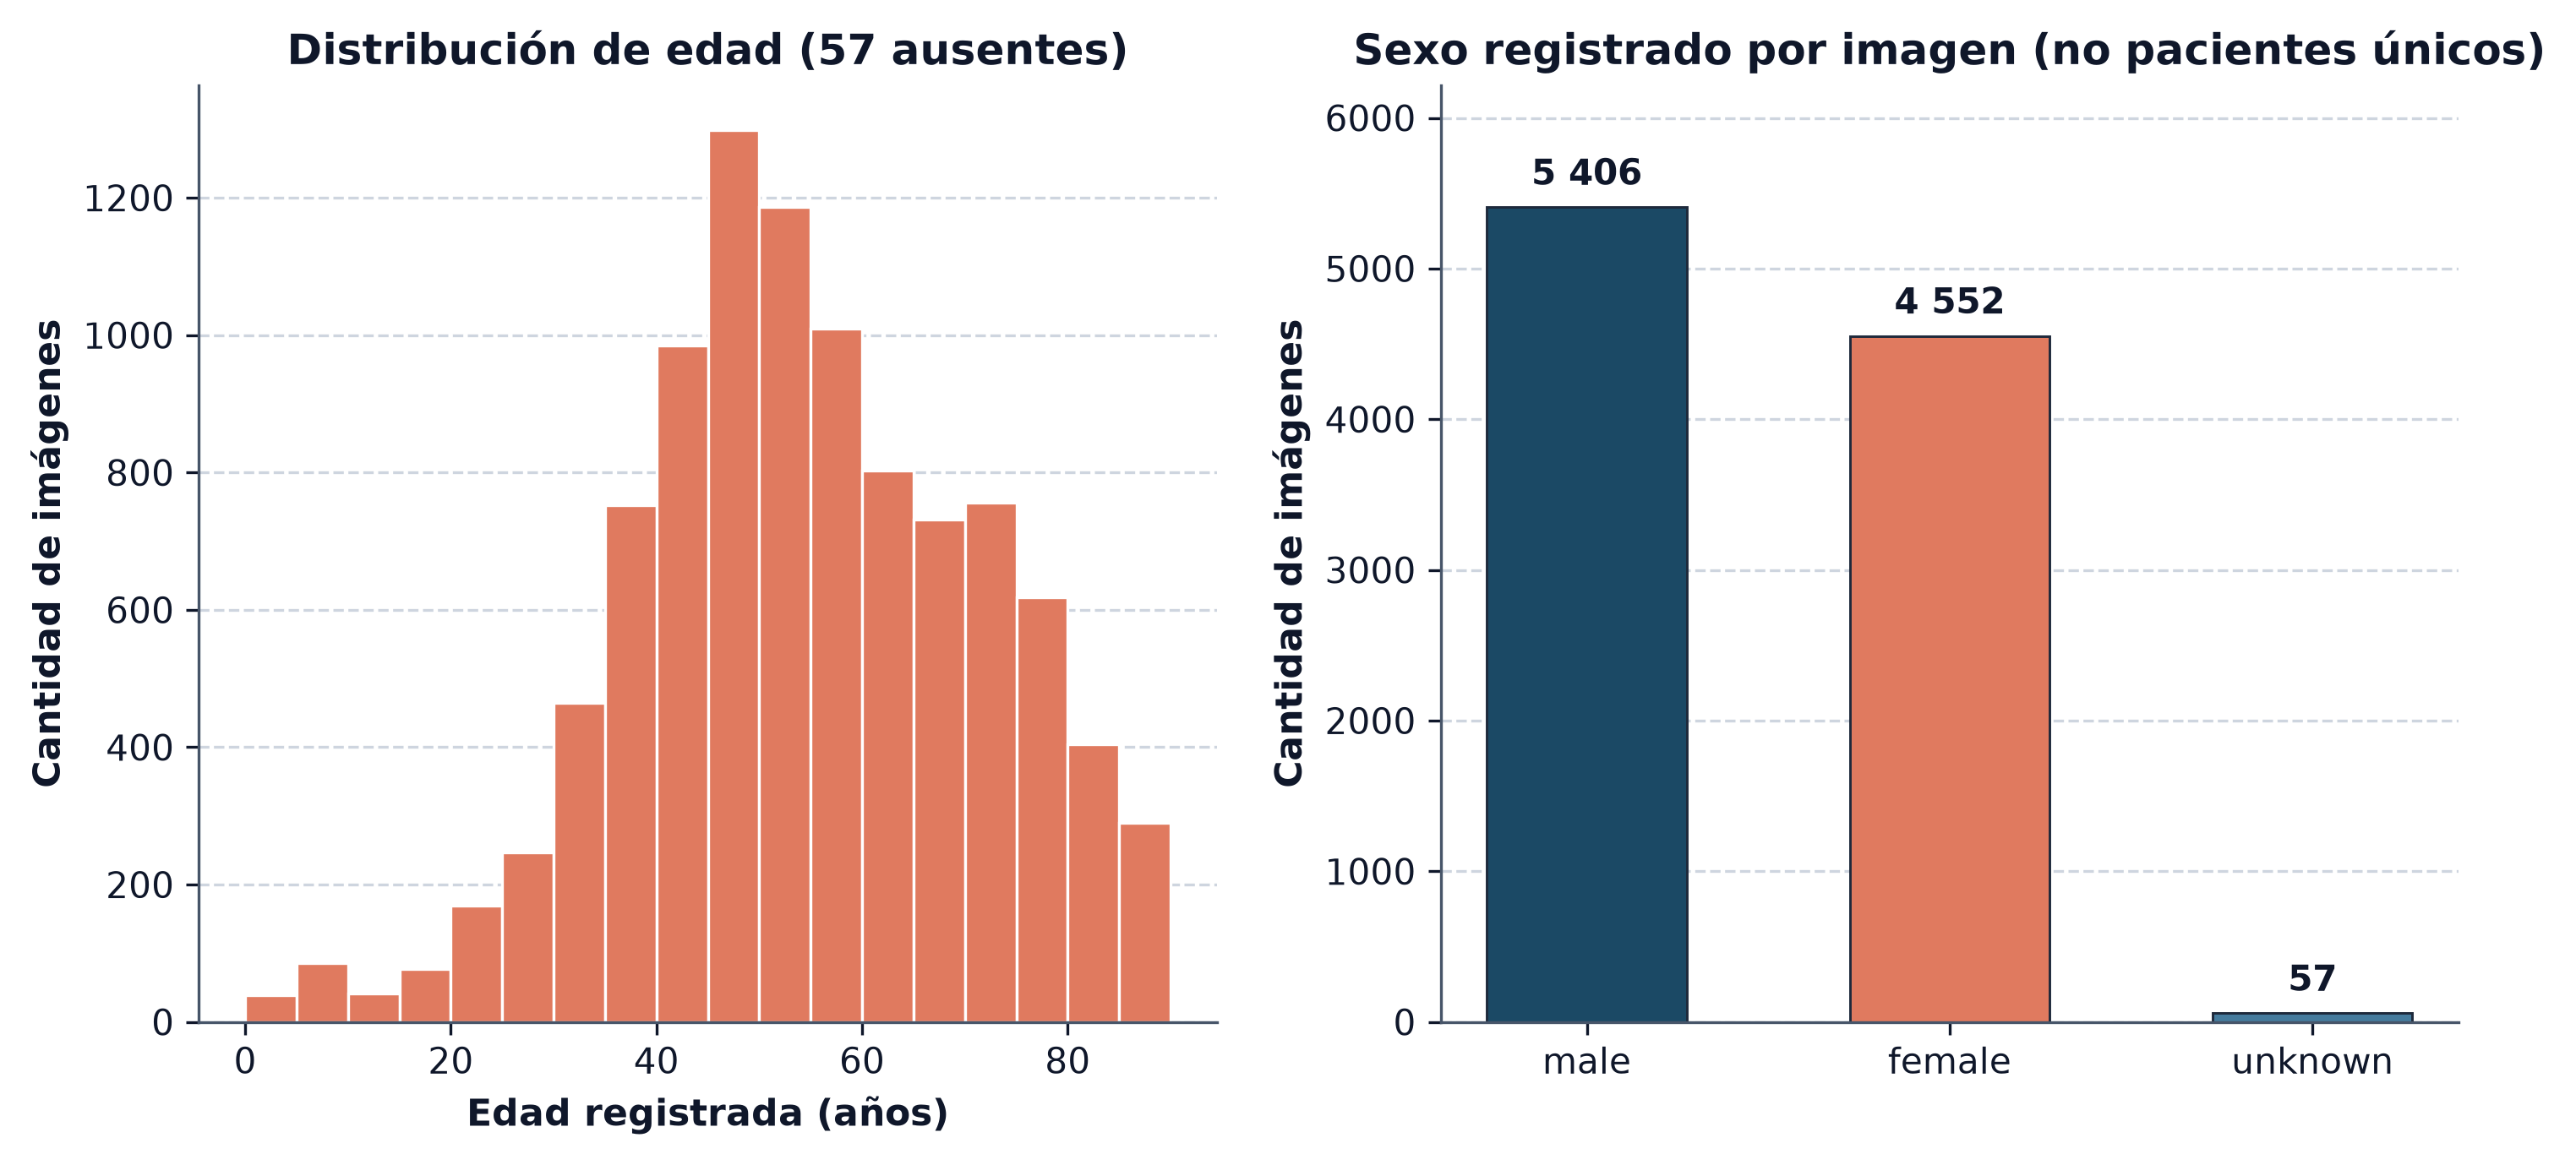
\includegraphics[width=0.92\textwidth]{06_metadata.png}
\caption{Distribución de edad y sexo registrados por imagen en HAM10000, con los 57 datos ausentes señalados explícitamente. Estas variables se describen pero no se añaden al clasificador principal.}
\label{fig:metadata}
\end{figure}

\begin{figure}[htbp]
\centering
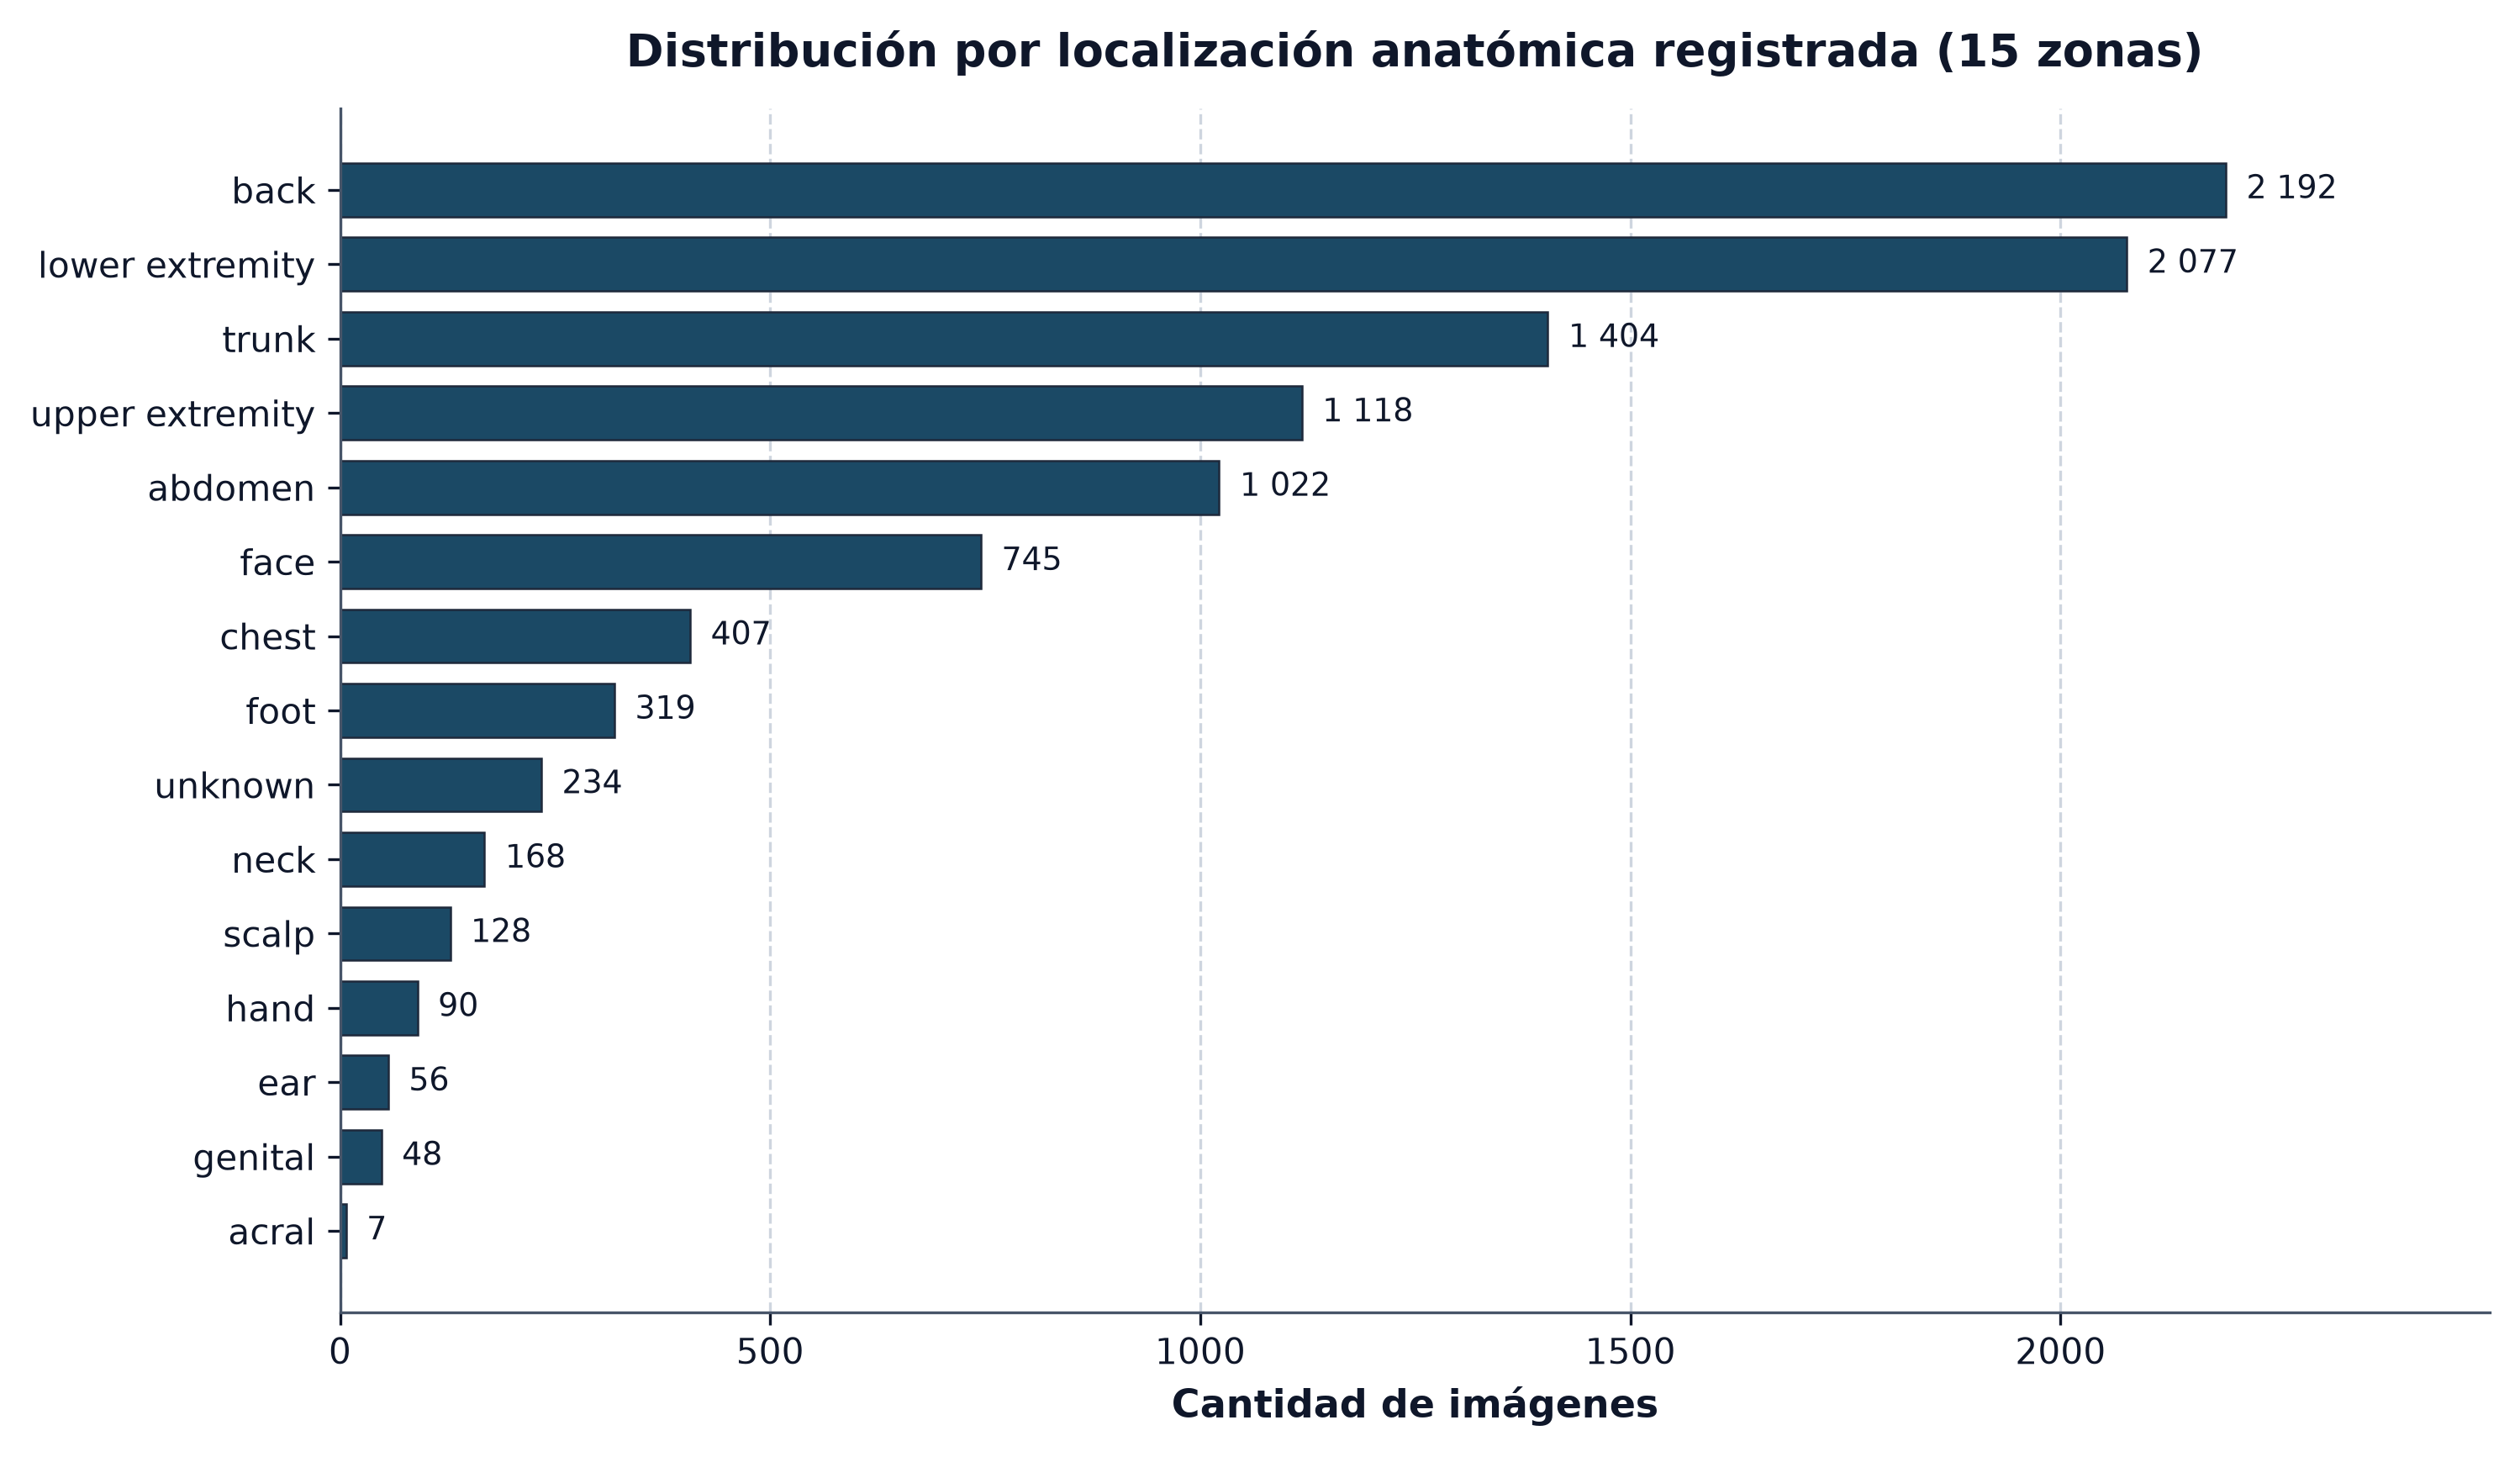
\includegraphics[width=0.92\textwidth]{07_localizacion.png}
\caption{Distribución de localización anatómica en 15 categorías registrada en el metadata de HAM10000 ($n=10\,015$ imágenes). Variable descriptiva no empleada como entrada del clasificador principal.}
\label{fig:localizacion}
\end{figure}
\FloatBarrier
